\documentclass{bhcguides}

\usepackage[legalpaper, portrait, margin=1.2in]{geometry}
\usepackage[utf8]{inputenc}
\usepackage{tabu}
\setlength{\parindent}{0pt}
\setlength{\parskip}{6 pt}

\usepackage{graphicx}
\graphicspath{ {images/} }

\usepackage{url}
\usepackage{hyperref}
\usepackage{cite}

\begin{document}

\title{Administrator Manual}

\includegraphics[width=1.0\textwidth]{BHCbanner.png}
\date{\today}
\maketitle

\tableofcontents

\section{Overview}

The Building Healthy Communities programme is a partnership that delivers a range of initiatives, activites, interventions and skills classes to improve the wellbeing of the community as a whole, and the members of that community. As an administrator, you have access to the inner workings of the system, to view and collate metrics on how well the programme is running, and the ability to create and manage initiatives across the Area Partnerships. But if you've come this far, you already know that. What you want to know is, what's this website got to do with anything, and how do I use it? That's where this manual comes in.

The Building Healthy Communities web system is a way to give you, the administrator, the power to easily and simply manage all the data driven aspects of the BHC programme from one consistent location. The service users and volunteers each use other sections of the system, with all their data feeding through to you, where you can view it in the manner you wish. Data can be viewed from the initiative level, through funding, all the way down to the details of individual service users and volunteers, and can be viewed in tables, searched, and downloaded for use elsewhere. Feedback is also integrated into the system, allowing you to track the efficacy of initiatives and the welfare of service users. This manual will walk you through the use of the system, and introduce you to the various features and intricacies of the system, giving examples as we go.

\section{System Access and Login}
\label{sec:syslogin}

The system is currently hosted at \url{http://hidden-mountain-49766.herokuapp.com} , which can be accessed through most major web browsers (Chrome, Firefox, Safari, IE8 or higher). Before accessing the system, you should have your email address and password on hand. If you are a new administrator, who has not previously accessed the system, you should ask another administrator to create an account for you. Upon entering the system, you will be taken to the login page, as seen in \autoref{fig:initialLogin}.

\begin{figure}[h!]
 \centerline{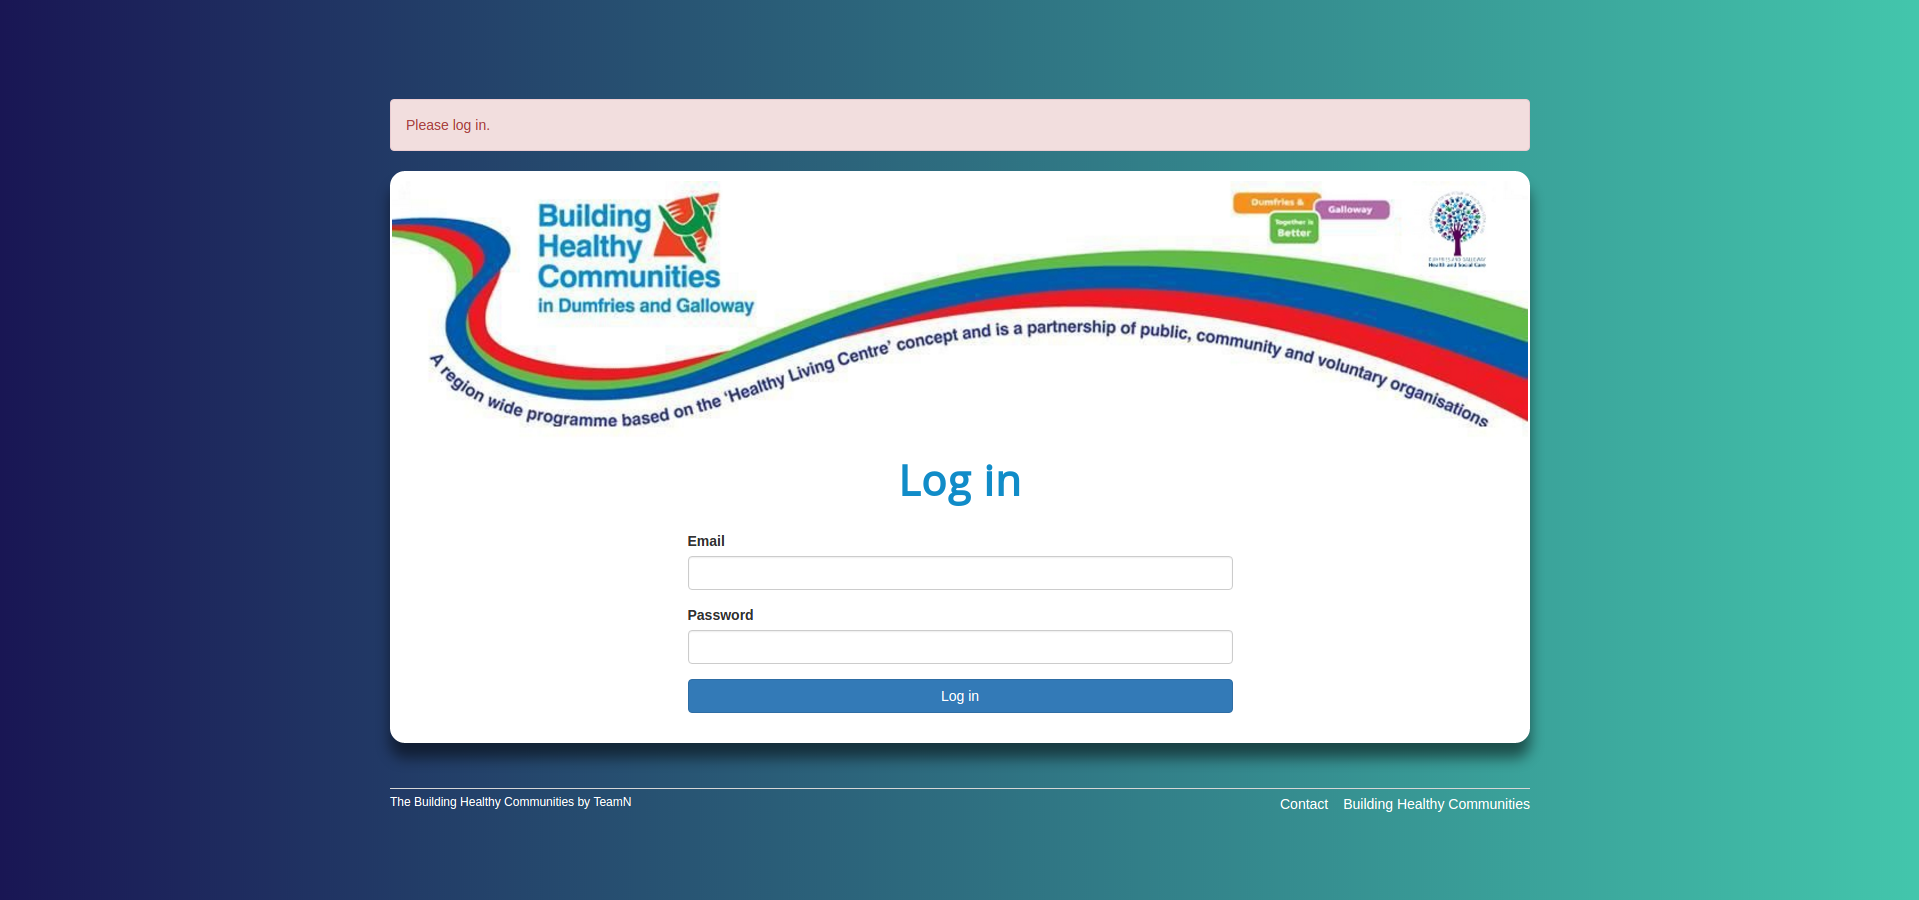
\includegraphics[width=\textwidth, height=\textheight, keepaspectratio]{loginscreen.png}}
 \caption{Login page}
 \label{fig:initialLogin}
\end{figure}

To login to the system, enter your email address and password. Until you do so, there is no way to gain access beyond this page. In the case that you have forgotten your email address and/or password, see \autoref{sec:contacts}: Contacts and Forgotten Passwords.

\pagebreak

\section{Menu Bar}
\label{sec:menubar}

The menu bar is a persistent feature, appearing at the top of every page on the system. It is designed to allow quick access to every major area of the site. The bar is split in two parts; a collection of links to the most commonly used parts of the system, and a drop down menu of links to the lesser used sections. Every link leads to its matching data table, except for Home and Profile, which lead to the home page and your profile page, respectively. There is also a Log out button that will log you out and return you to the login screen.

\begin{figure}[h!]
 \centerline{
\includegraphics[width=\textwidth, height=\textheight, keepaspectratio]{menubar.png}}
 \caption{Menu bar with drop down}
 \label{fig:initialLogin}
\end{figure}

\section{Home Page}
\label{sec:homepage}

Upon logging in to the system, the first page that will be loaded is the home page. This page is a quick overview of the system, presenting groups of useful information and allowing you to quickly navigate and execute a few simple actions. The home page is split into three sections: the Area Overview, Statistics, and Service Requests.

\subsection{Area Overview}
\label{ssec:areaoverview}

The Area Overview is the first major feature on the website home page. From here you can quickly see the names of every initiative run by each area partnership. Clicking the name of an area will take you the relevant area page, and clicking an initiative name will do so for relevant initiative. For more information on areas and initiatives see \autoref{sec:areas}: Areas and \autoref{sec:initiatives}: Initiatives.

\begin{figure}[h!]
 \centerline{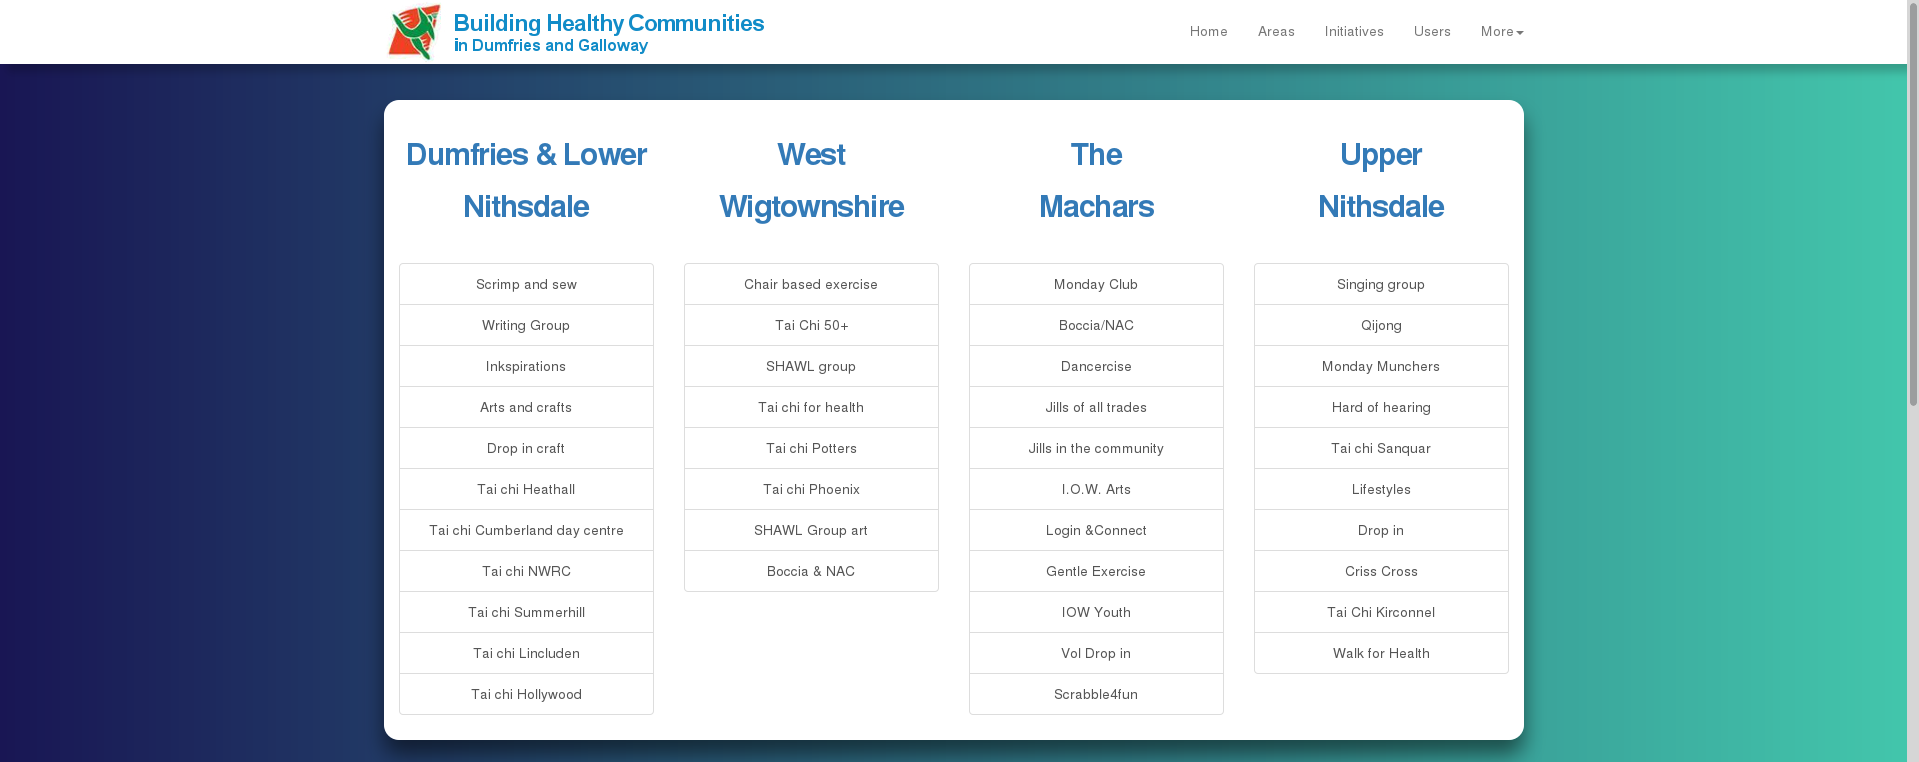
\includegraphics[width=\textwidth, height=\textheight, keepaspectratio]{homepage1.png}}
 \caption{Area Overview}
 \label{fig:homePage1}
\end{figure}

\subsection{Statistics}
\label{ssec:statistics}

The Statistics section is a quick rundown of the status of the system as a whole. It features a small collection of information, including:

\begin{itemize}
	\item The total number of service users, volunteers, and funders
	\item The most and least popular initiatives (those with the highest and lowest number of members)
	\item The most and least assigned medical conditions
	\item A graph of the total monthly attendance across all initiatives over the last 2 years
	\item A graph of the average monthly attendance as a percentage, over the same period as above.
\end{itemize}

Clicking the name of an initiative or condition will take you to the relevant details page.

\begin{figure}[h!]
 \centerline{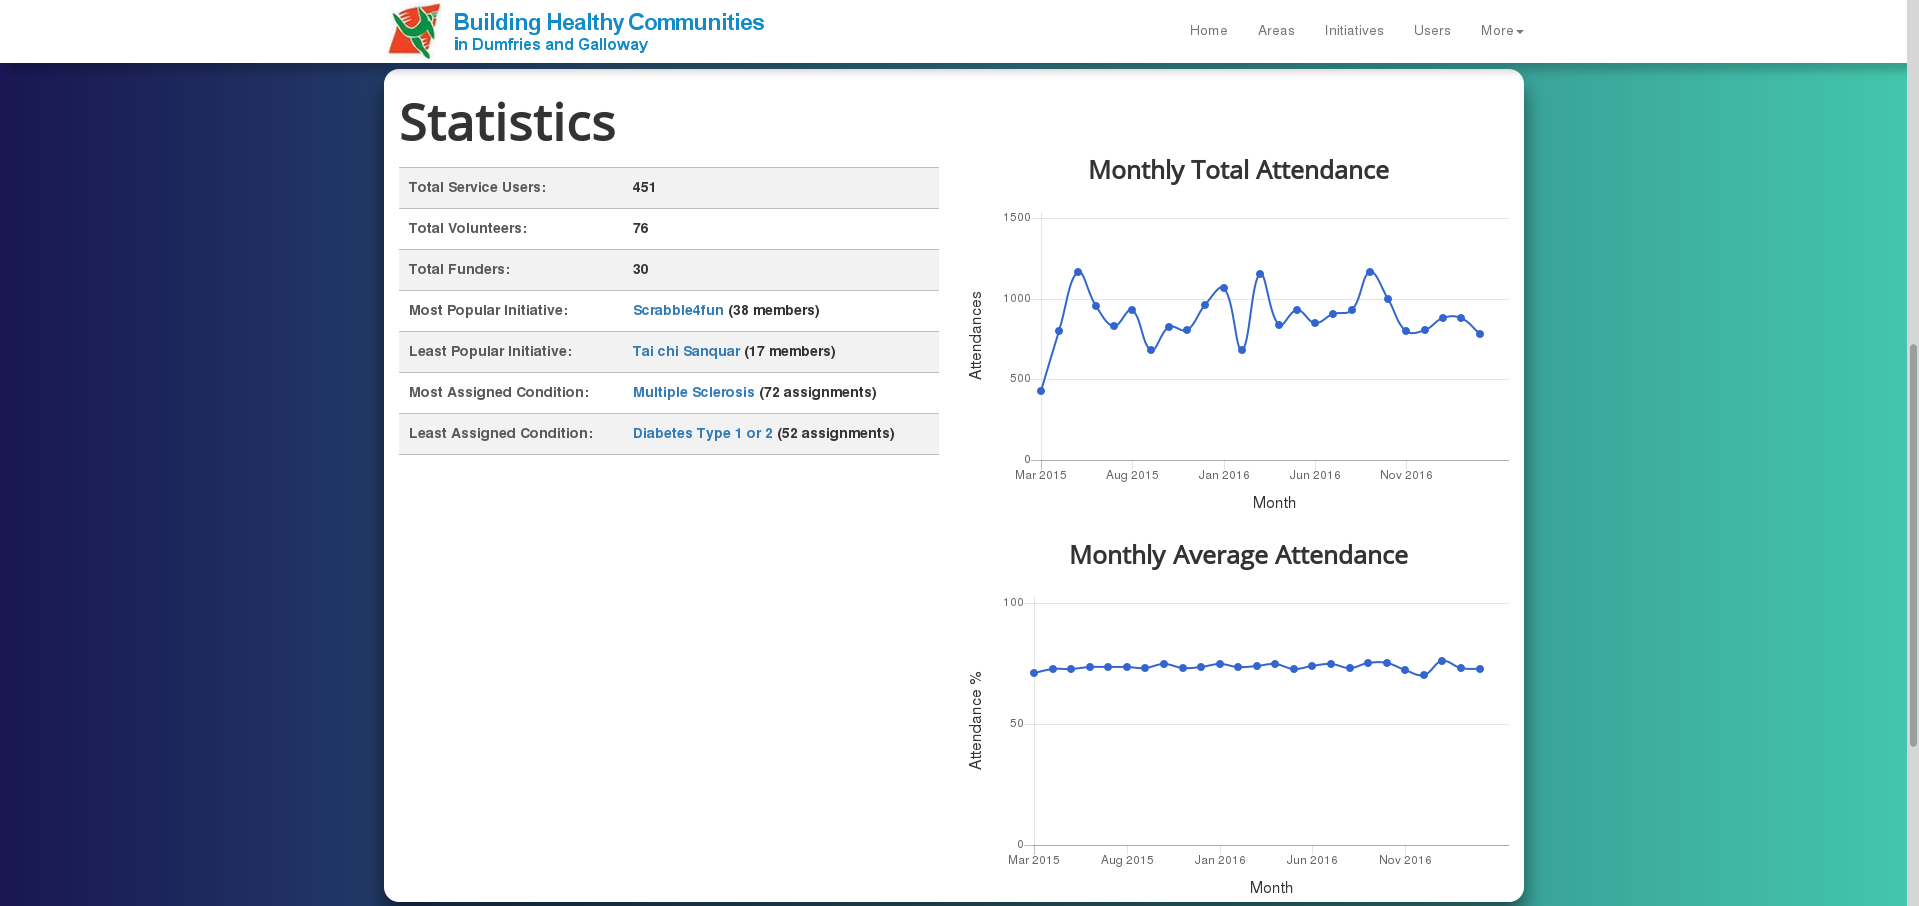
\includegraphics[width=\textwidth, height=\textheight, keepaspectratio]{homepage2.png}}
 \caption{Statistics}
 \label{fig:statistics}
\end{figure}

\subsection{Service Requests}
\label{ssec:servicerequests}

The service requests section allows you to see all the messages sent to you by service users ad volunteers asking you to change their details. To change their details, open the user's profile, change the relevant details (described in more details in \autoref{sec:users}: Users, and save them. You can then delete the service request.

\begin{figure}[h!]
 \centerline{
\includegraphics[width=\textwidth, height=\textheight, keepaspectratio]{homepage3.png}}
 \caption{Service Requests}
 \label{fig:serviceRequests}
\end{figure}

\section{Profile}
\label{sec:profile}

\section{Data Tables}
\label{sec:datatables}

\section{Areas}
\label{sec:areas}

\section{Initiatives}
\label{sec:initiatives}

\section{Users}
\label{sec:users}

\section{Medical Conditions}
\label{sec:medical}

\section{Questions}
\label{sec:questions}

\section{Funders}
\label{sec:funders}

\section{Meetings}
\label{sec:meetings}

\section{Archives}
\label{sec:archives}

\section{Contacts and Forgotten Passwords}
\label{sec:contacts}

If you want to find contact details for a given area, there is an easy way to do so. On the login page (you will have to log out if you are currently logged in), in the bottom right is the word 'Contact'. Clicking on this will bring up the contacts page, from which the addresses of the various area partnerships can be found, as seen in \autoref{fig:contactPage}. This page also includes the names and roles of people working there, and a telephone number. If you have forgotten your email address and/or password, then you should contact another administrator directly, as the situation could pose a security risk. Other administrators can reset your account details, but should only do so with your explicit authorisation.

\begin{figure}[h]
 \centerline{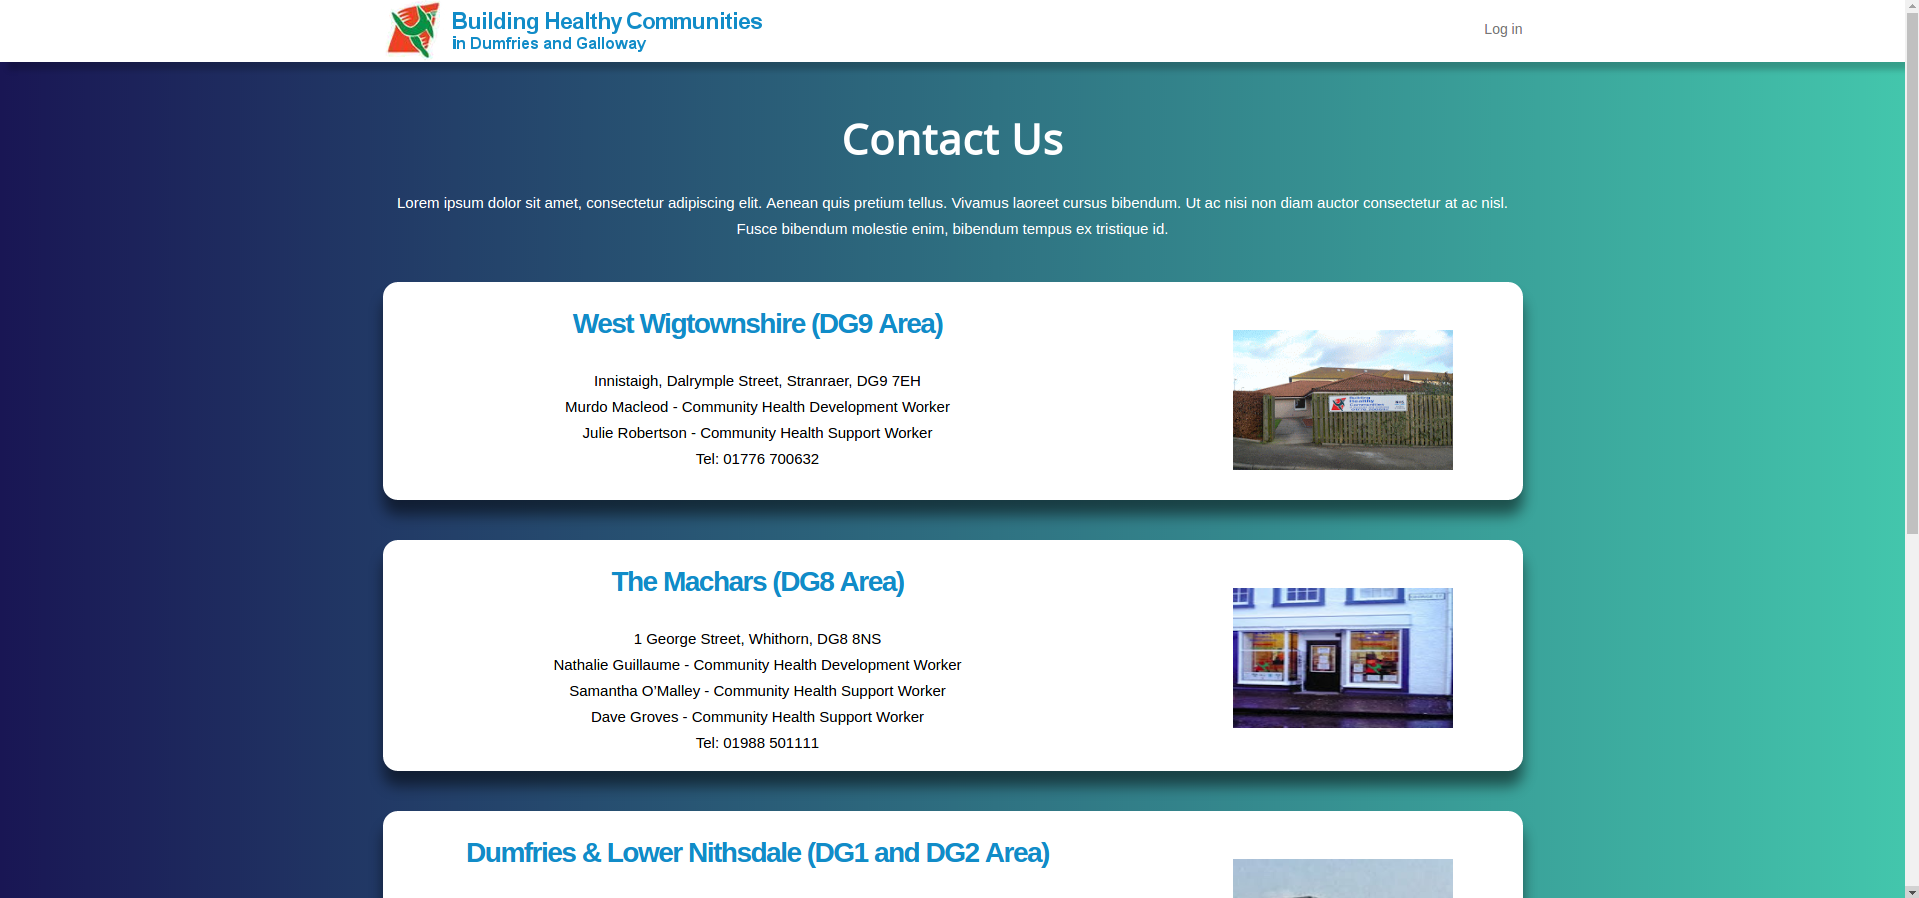
\includegraphics[width=\textwidth, height=\textheight, keepaspectratio]{contactpage.png}}
 \caption{Contact page}
 \label{fig:contactPage}
\end{figure}

\end{document}
